%%% LaTeX Template: Article/Thesis/etc. with colored headings and special fonts
%%%
%%% Source: http://www.howtotex.com/
%%% Feel free to distribute this template, but please keep to referal to http://www.howtotex.com/ here.
%%% February 2011
%%%
%%% Modified October 2015 by CDM

%%%  Preamble
\documentclass[11pt,letterpaper]{article}
\usepackage[margin=1.0in]{geometry}
\usepackage[T1]{fontenc}
\usepackage[bitstream-charter]{mathdesign}
\usepackage[latin1]{inputenc}					
\usepackage{amsmath}						
\usepackage{xcolor}
\usepackage{cite}
\usepackage{hyphenat}
\usepackage{graphicx}
\usepackage{float}
\usepackage{subfigure}
\usepackage{sectsty}
\usepackage[compact]{titlesec} 
\usepackage[tablegrid]{vhistory}
\allsectionsfont{\color{accentcolor}\scshape\selectfont}

%%% Definitions
\definecolor{accentcolor}{rgb}{0.0,0.0,0.5} 
\newcommand{\teamname}{Team 2}
\newcommand{\productname}{RFID Automated Student Dismissal}
\newcommand{\coursename}{CSE 4316: Senior Design I}
\newcommand{\semester}{Fall 2017}
\newcommand{\docname}{Project Charter}
\newcommand{\department}{Department of Computer Science \& Engineering}
\newcommand{\university}{The University of Texas at Arlington}
\newcommand{\authors}{Bibek Khatakho \\Austin Hastings \\ Kashif Iqbal \\ Nupur Pandey \\ Albaro Tonoco}

%%% Headers and footers
\usepackage{fancyhdr}
	\pagestyle{fancy}						% Enabling the custom headers/footers
\usepackage{lastpage}	
	% Header (empty)
	\lhead{}
	\chead{}
	\rhead{}
	% Footer
	\lfoot{\footnotesize \teamname \ - \semester}
	\cfoot{}
	\rfoot{\footnotesize page \thepage\ of \pageref{LastPage}}	% "Page 1 of 2"
	\renewcommand{\headrulewidth}{0.0pt}
	\renewcommand{\footrulewidth}{0.4pt}

%%% Change the abstract environment
\usepackage[runin]{abstract}			% runin option for a run-in title
%\setlength\absleftindent{30pt}			% left margin
%\setlength\absrightindent{30pt}		% right margin
\abslabeldelim{\quad}	
\setlength{\abstitleskip}{-10pt}
\renewcommand{\abstractname}{}
\renewcommand{\abstracttextfont}{\color{accentcolor} \small \slshape}	% slanted text

%%% Start of the document
\begin{document}

%%% Cover sheet
{\centering \huge \color{accentcolor} \sc \textbf{\department \\ \university} \par}
\vspace{0.5 in}
{\centering \huge \color{accentcolor} \sc \textbf{\docname \\ \coursename \\ \semester} \par}
\vspace{0.5 in}
\begin{figure}[h!]
	\centering
   	
\includegraphics[width=0.60\textwidth]{./images/test_image.jpg}
\end{figure}
\vspace{0.5 in}
{\centering \huge \color{accentcolor} \sc \textbf{\teamname \\ \productname} \par}
\vspace{0.5 in}
{\centering \large \sc \textbf{\authors} \par}
\newpage


%\vspace{1 in}
%\centerline{January 13th, 2012}
%\newpage

%%% Revision History
\begin{versionhistory}
  	\vhEntry{0.1}{10.06.2017}{AH}{document creation}
	\vhEntry{0.2}{11.12.2017}{BK, AH, NP, AT}{document revision}
	\vhEntry{0.3}{11.19.2017}{AH, NP, AT}{document revision}
	\vhEntry{1.0}{12.10.2017}{BK, AH, KI, NP, AT}{document revision}

\end{versionhistory}
\newpage

%%% Table of contents
\tableofcontents
\newpage

%%% Agile project charter sections
\section{Vision}
\quad \quad For parents that pick up their children from school, it is often a long and tedious process. Pulling into the designated lane amongst several other parents and their vehicles, having a staff member verify who they are, whom you are picking up and then calling out your child's name over the radio to finally have them get ready to leave the building with all their belongings.  To address this concern, we are building an automated system that will verify who has arrived, what student needs to be made ready for dismissal and to send that information over to a centralized location for staff to streamline dismissal. 
\section{Mission}
\quad \quad The primary mission of this project is to replace traditional method of picking children from school. The system will use Rfid scanner to scan the incoming vehicle of parents of the children in school. The application that run in windows will process the information collected by scanner. The Rfid scanner scan the vehicle with rfid sticker and display the information of the parents and children in the gui. The interactive gui will show the list of information of children whose parents have arrived. The list will be updated as new vehicle is detected by the scanner. The application will show the names of students who have left and who have not left from school on that particular day. The application will also save the information in database for future reference.

\section{Success Criteria}
\quad \quad This project will be considered successful if the outcome is able to replicate the core functionalities of the current staff employee's dismissal duties by the RFID reader. 
Namely, the ability to relay arriving parents notice to the correct staff members who have authorization to dismiss that parent's child. 
The goal will require the construction of a RFID reader, housing, and mount connected to the system which will not succumb to outside elements. 
A successful example would be that the parents drive by with a RFID Tag placed on the windshield of their vehicles, the RFID reader, reads the tag and sends that notice to the system database to query and recover all associated information for the staff member to confidently release/dismiss the child that belongs to that parent all before the parent arrives to the pickup area.

\newpage

%%% Remaining project charter sections
\section{Background}
\quad \quad The idea for this project was addressed by the professor to the group. 
One of the professors on campus had to go pick up her kid from school. There the 
parents take a paper with the child's name so that the employees at school knew who 
the parent want to pick up. This method is slow as parents had to wait for a while 
before they saw their children, it is not convenient for the school employees as they 
had to adjust for all sort of weather and it is not safe for the child as people with 
evil intentions can have access to kids name.
The team decided to take on this project because we realized that the concern is 
serious and if we can finish the project and bring it in-front of schools they will be 
able to use it. This will not only benefit us as students rather the parents, kids, 
employees at school as well as school. This project has real-world benefit and can be 
used in multiple fields. For example, this project can be used at a fast food place as 
well as customers can order using their phone where they can enter their license plate 
number and when they come inside the field of fast food place, the fast food employee 
can bring their food out right away after the scanner reads their license plate. 
Analyzing the wide range of fields where this project can be used in real world and 
the positive impacts that it can have on people and businesses, we have chosen this 
project.
\section{Related Work}
\quad \quad There are similarly related applications for schools to utilize that would 
help with tracking the students at various times of uncertainty such as when the 
students travels by bus and when they arrive at school.
The related commercially available products are listed below:
\begin{itemize}
	\item http://www.laconictechnology.com/education-sector.html - School Bus 
	Attendance Model (GPS + RFID), Basic GPS Tracking Systems, GPS + RFID Systems.
	\item http://northstar.global/rfid-school-bus-tracking-system/ - Northstar's RFID 
	system helps track the movement of children in schools and verifies if students 
	are getting off at the right bus stop. It also helps automate attendance.
	\item http://rfid.thingmagic.com/rfid-blog/bid/50802/RFID-for-Student-Tracking - 
	he benefits of RFID-enabled student tracking solutions are providing secure access 
	to a building and recording attendance.
\end{itemize}
\quad \quad These systems are primarily put in place for when the students arrive or 
when they board transportation provided by the school for parents to have SMS updates 
sent to their phones in real time. Our project will utilized the same technology but 
only focus on the dismissal tracking for students so that the system automates what 
child needs to be made ready for dismissal whenever their parent has arrived and is 
ready to pick up their child. 
\section{System Overview}
\quad \quad The overall structure of the software system contains three layers: Student Management 
System, DataBase, and Queue Display System. The Student Management System is user end 
system which is related to administrative functionality that includes adding, removing 
and editing student and staff information in the system. The GUI allows the admin to 
add student and remove student. The DataBase System is responsible for storing the 
information. It also allows the user to make queries. The Queue Display System displays 
the information of the system and also handles the RFID listener. This is a user end 
system and also includes hardware. The Queue Display System and Database System 
communicate with each other to keep real time records of the student pickup.

\begin{figure}[h!]
	\centering
 	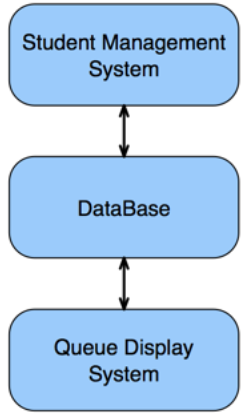
\includegraphics[width=0.40\textwidth]{images/ads_1}
 \caption{Overall Structure of System}
\end{figure}

\subsection{Student Management System Layer Description}
\quad \quad The Student Management System includes a control system, database control, and GUI. 
Control. This System directly talks with the Database System in order to store all the 
information about the students.

\subsection{Database Layer Description}
\quad \quad This System contains the tables to store the text and image of the system. Database 
System directly talks with Student Management System and Queue Display System.

\subsection{Queue Display System Layer Description}
\quad \quad This System contains control system, dbcontrol, GUI and RFID API. The RFID API helps 
to maintain communication between the Queue Display System and the RFID reader. The 
GUI displays the list of the students as their parents approach the school.
\section{Roles \& Responsibilities}
\quad \quad Kashif Iqbal is the System Architect. Kashif is one of the two Software 
Engineers in our team, he has been exposed to 10 different languages throughout his 
academic time here at UTA. Some of the coursework that he is currently taking which 
includes Design Patterns and Object Oriented Software Engineering (Agile Methodology) 
would be very useful for our Senior Design project. He has extensive knowledge of 
Python, C/C++, Java and MySQL which will most likely be the grounds for this project. 
He is in charge of picking the Design Patterns, relevant libraries, the Database Model, and the Model Infrastructure. 
He will extract the RFID information from the reader and relay it down the pipeline. 
\par 
Bibek Khatakho is the Front End Developer. 
He has also taken ARTS class and some design courses which will help him to design 
interactive GUI for the project. He is proficient with C++, Java, and Python.
He will design the user interface. This includes the Sign-in page, the Admin page, and 
the generic Staff page. 
\par 
Albaro Tinoco is the Hardware Integrator. 
Always being on time and ready to work whenever the scheduled time is. He strives to 
make the working environment likeable by keeping our spirits high by having 
conversations and making compromises. His programming development skills experience 
comes from working on school projects. He is interested in GUI based front-end 
applications and making videogames with extensive knowledge in Python, C/C++, Java and 
MySQL. He will connect the reader to the computer physically and design hardware to 
support the scanner off the ground. 
\par 
Austin Hastings is in charge of documentation, will help with 
debugging and is Scrum Master. He is experienced with Java, Matlab, and Python. He also 
has knowledge in C, C++, C\#, and SQL. He is interested in Cyber Security and will make 
sure the system is as secure as possible. As Scrum Master, he is in charge of 
establishing sprint goals.
\par 
Nupur Pandey is the Back End Developer. 
He has work experience with MS- SQL. He has also worked as a back end developer for 
multiple projects here on campus. He has extensive knowledge of Python, C\#, C/C++, 
Java and MySQL which will most likely be the grounds for this project. 
He is in charge of generating the database schema, scripts and formatting queries.
\section{Facilities \& Equipment}
\quad \quad The development and prototyping of RDF student pick-up will take place 
in Senior Design Lab. All the hardware design and development will take place in the 
lab during Senior Design I. We have received the RFID reader from the school. 
We will also be using common tools such as the drills, screwdrivers, saws, and allen 
wrenches from the Senior Design Lab. We may use a 3D printer as the need arises. 
Tools that are not available from the lab will be brought by our team with Professor's 
approval. Upon completion of the RFID student pick-up, we will be testing it at the 
senior design lab and parking lot of the school. 

\section{Cost Proposal}
\quad \quad We have \$800 provided by the Computer Science department of UTA for the project. At the moment, we do not have any financial donors for the project. We are going to use personal computer and the Rfid scanner for the lab, so we will not have much expenditure. We will spend approximately \$100 to buy the hardware to structure the system.

\subsection{Preliminary Budget}
\quad \quad Purchase Hardware: To recognize vehicle.
Purchase Hardware: To store database.
Purchase Hardware: To display results.

\subsection{Current \& Pending Support}
\quad \quad Purchased RFID Scanner.
\section{Documentation \& Reporting}
\quad \quad In this section, all of the various artifacts that are to be generaterated and 
maintained are described.

\subsection{Project Charter}
\quad \quad The Project Charter is this document. It will be updated as major changes are 
updated, and will provide a guiding backbone for the progress of this project.

\subsection{Product Backlog}
\quad \quad As product gets backlog, more manhours will be applied in importance order. This 
form will be used to designate what was expected to be accomplished, yet was not 
completed.

\subsection{Sprint Planning}
\quad \quad Sprints will be planned with all team members present at the beginning of all 
sprints. Changes to the expectations to a sprint will take place with at least a 
majority in concensus.

\subsubsection{Sprint Goal}
\quad \quad Sprint goals will generated during planning and rechecked before the end of each 
sprint. Failing to complete all tasks for a sprint goal will cause reevaluation of 
future deadlines and will be tracked in the product backlog.

\subsubsection{Sprint Backlog}
\quad \quad Sprint Backlogs will be re-evaluated and worthwhile actions will be added to 
subsequent sprints.

\subsubsection{Task Breakdown}
\quad \quad Tasks will be divided to each team member's specialities. Free members will be 
applied to Tasks overlapping or concurrent to busy team members.


\subsection{Sprint Retrospective}
\quad \quad Activities done during sprints will be reviewed and successful activites will be 
promoted to be attempted again. The retrospective will be a time of communication 
and free flowing of ideas.

\subsection{Individual Status Reports}
\quad \quad Individual Status Reports will be generated by each team member.

\subsection{Engineering Notebooks}
\quad \quad Engineering Notebooks will be kept by all team members and checked as needed to 
remain in regulation. Each team member is free to fill their notebook with relevant 
figures and information to complete their tasks.

\subsection{Closeout Materials}
\quad \quad Closeout Materials will we generated before the completion of the project. These 
materials include a \"How To demo\", product website, a product poster, and a video 
of use.

\subsubsection{System Prototype}
\quad \quad A working System Prototype will be implimented before May 2018.

\subsubsection{Project Poster}
\quad \quad A detailed Project Poster will be created before May 2018.

\subsubsection{Web Page}
\quad \quad A Web Page documenting the design process and related material may be created before 
May 2018.

\subsubsection{Demo Video}
\quad \quad A Demo Video will be created, showing the product in action, before May 2018.

\subsubsection{Source Code}
\quad \quad Source Code will be hosted on GitHub.

\subsubsection{Source Code Documentation}
\quad \quad Source Code Documentation will be taken care of by Doxygen.

\subsubsection{Hardware Schematics}
\quad \quad Hardware Schematics will be maintained as hardware is purchased or manufactured. 
These will be available upon project completion.

\subsubsection{CAD files}
\quad \quad CAD files will be hosted on GitHub.

\subsubsection{Installation Scripts}
\quad \quad Installation Scripts will be installed to hardware before reaching the site.

\subsubsection{User Manual}
\quad \quad A User Manual will be created and either available on the website or in physical copy.
\newpage

%%% References
\bibliographystyle{plain}
\bibliographystyle{reference/IEEEtran_custom}
\bibliography{reference/refs}{}

\end{document}